%Diese LaTeX-Vorlage f�r Praktikumsprotokolle in Form einer Ver�ffentlichung f�r das 
%F-Praktikum wurde erstellt von Andreas Nuber EP II, Uni W�rzburg.
%Es wurde das Koma-Skript verwendet und sollte somit installiert sein
%desweiteren sollten alle packages installiert sein, die mit \usepackage{} 
%eingebunden werden.
%Zum Testen dieser Vorlage wurde MikTex verwendet sowie TeXnicCenter als Editor
%beim Compilieren waren 0 Fehler, 1 Warnung und 3 zu volle/leere Boxen. Das ist ok :)

%F�r das Erstellen einfach den sinnfreien Text, der zum ausf�llen genommen wurde 
%ersetzen. Was sonst noch ver�ndert werden sollte steht in den Kommentaren!


\documentclass[a4paper,10pt,twocolumn]{scrartcl} %Koma-Skript-�quivalent zu "article"

\usepackage{german}            %macht deutsche �berschriften
\usepackage{amsmath}           %macht
\usepackage{amsfonts}          %       Mathe
\usepackage{amssymb}           %              m�chtiger
\usepackage{graphicx}          %erlaubt Graphiken einzubinden (.eps f�r dvi und ps sowie .jpg f�r pdf)
\usepackage[T1]{fontenc}       %Zeichenbelegung der verwendeten Schrift
\usepackage{ae}                %macht sch�neres �
\usepackage{typearea}	         %erm�glicht �nderung des Seitenspiegels
\usepackage{scrlayer-scrpage}          %erm�glicht �nderung der Kopf-/Fu�zeile
\usepackage{lastpage}          %l�sst auf die Seienanzahl zugreifen
\usepackage[margin=10pt,font=small,labelfont=bf]{caption} %macht die Bildbeschriftungen richtig

\renewcommand{\figurename}{Abb.}

\pagestyle{scrheadings}        %sagt Koma-Skript, dass selbstdefiniers Kopfzeilen verwendet werden
\typearea{16}                  %stellt Seitenspiegel ein
\columnsep25pt								 %definiert Breite zwischen den zwei Spalten von \twocolumns

\renewcommand{\pnumfont}{%     %�ndert die Schriftart der Seitennummerierung
\normalfont\rmfamily\slshape}  %�ndert die Schriftart der Seitennummerierung 



\begin{document}
\cfoot{\thepage /\pageref{LastPage}}     %macht die Seitennumerierung der Fom 2/5 (ausser auf der Titelseite)

\twocolumn[{\csname @twocolumnfalse\endcsname                %erlaubt "Abstrakt" �ber beide Spalten
\titlehead{                                                  %Kopfzeile
	\begin{tabular*}{\textwidth}[]{@{\extracolsep{\fill}}lr}   %Kopfzeile
	Betreuer: Der Betreuer & \today\\                          %Kopfzeile      hier den Betreuer eintragen!!!
	\end{tabular*}                                             %Kopfzeile
	}
\title{Festk\"orperoptik: Bandparameter und optische Konstanten}  %Titel der Versuchs
\author{Name Student 1 und Name Student 2}                     %Namen der Studenten
\date{}                                                         %ben�tigt um automatisches Datum auszuschalten
\maketitle                                                      %erzeugt Titelseite
\vspace{-8ex}                                                   %verringert Abstand zur �berschrift
\begin{abstract}                                                %Beginn des Abstracts
Fusce urna magna,neque eget lacus. Maecenas justo urna, lacinia vitae, vesti. Cras erat. Aliquam pede. vulputate e dolor ac adipiscing amet bibendum nullam, massa lacus molestie ut libero nec, diam et, sodales eget, feugiat ullamcorper id tempore. Ac dolor ac adipiscing amet bibendum. Maecenas felis nunc, aliquam ac, consequat vitae, feugiat at, blandit vitae, euismod vel, nunc. Aenean ut erat ut nibh commodo suscipit. . Ac dolor ac adipiscing amet bibendum. Maecenas felis nunc, aliquam ac, consequat vitae, feugiat at, blandit vitae, euismod vel, nunc. Aenean ut erat ut nibh commodo suscipit.  
\\ \\ 
\\ 
Versuchsdurchführung: 02. Februar 2006\\       %Datum �ndern!
Protokollabgabe: 01. März 2006                 %Datum �ndern!
\\ 
\\ 
\end{abstract}
}]

\section{Einleitung}


\section{Theorie}
\begin{align}
T+R+A=1
\end{align}

\begin{align}                          %Beispiel wie man eine Gleichung TeXt
R=\left|\frac{n-1}{n+1}\right|^2
\end{align}

\section{Experiment}

\begin{figure}[htbp]                                 %So bindet man Graphiken ein
\begin{center}                                       %zentriert die Graphik
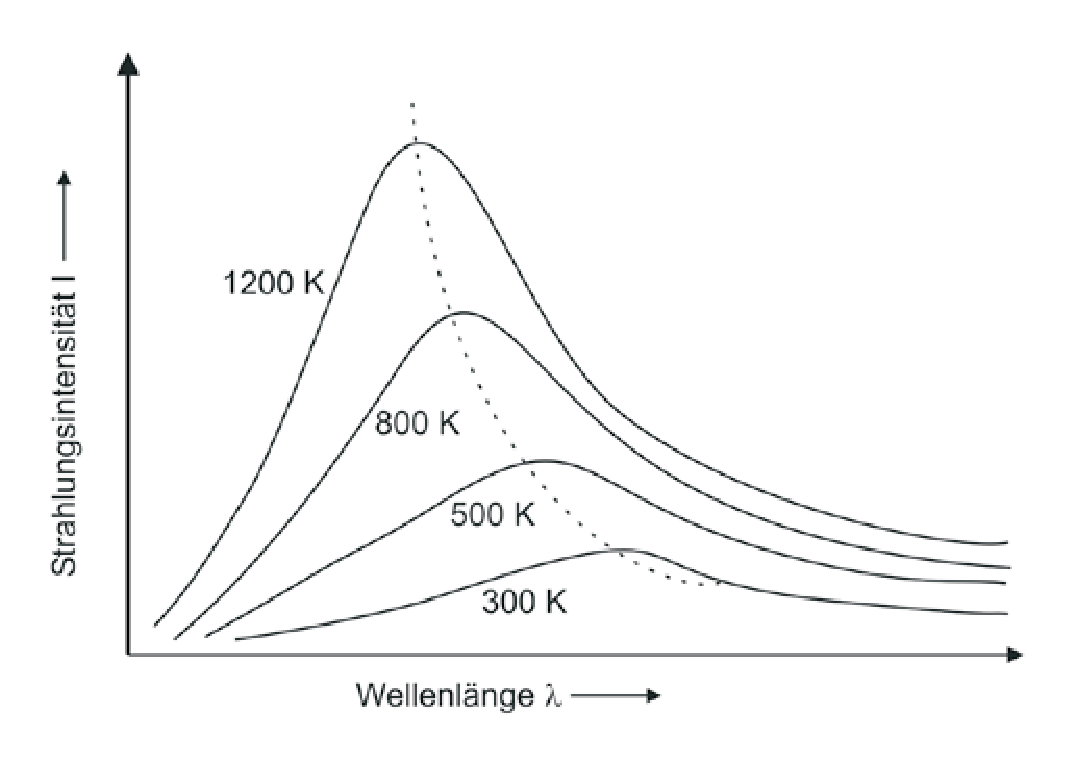
\includegraphics[width=0.9\linewidth]{bild1}       %das eingentliche Einbinden; "schwarz" ist der Dateiname ohne Endung
\caption[]{}   %Beschriftung der Graphik
\label{schwarz}                                      %das wird zu Zitiern im Text gebraucht
\end{center}
\end{figure}

\section{Auswertung}

\begin{table}[htbp]          %so funktionieren die Tabellen in LaTeX
\centering
\begin{tabular*}{\linewidth}{@{\extracolsep{\fill}}ccc}
\hline
\hline
\rule[-7pt]{0pt}{23pt}  Subshell  &     $j$ values 						  		&     Area ratio \\
\hline
\rule[-6pt]{0pt}{21pt}   $s$ 			&     $\frac{1}{2}$ 							&       --- \\

\rule[-6pt]{0pt}{21pt}   $p$ 			&     $\frac{1}{2},\frac{3}{2}$ 	&     $1:2$ \\

\rule[-6pt]{0pt}{21pt}   $d$ 			&     $\frac{3}{2},\frac{5}{2}$ 	&     $2:3$ \\

\rule[-7pt]{0pt}{22pt}   $f$ 			&     $\frac{5}{2},\frac{7}{2}$ 	&     $3:4$ \\
\hline
\hline
\end{tabular*}  
\caption[]{}  %siehe Graphik: Beschriftung
\label{spinsplit}                             %siehe Graphik: zum Zitieren
\end{table}

\section{Zusammenfassung}

\begin{thebibliography}{}    %so wird das Literaturverzeicnis erstellt
\bibitem{a}
\bibitem{b} 

\end{thebibliography}



\end{document}